\documentclass[a6paper,landscape,10pt]{report}

\usepackage[utf8]{inputenc}
%\usepackage{xltxtra}
\usepackage[portuguese]{babel}
\usepackage[top=1cm,left=.4cm,right=.4cm,bottom=.8cm,footskip=0cm]{geometry} %Define margens e distância do rodapé
\usepackage{titletoc} %Para definir o estilo da lista de conteúdo
\usepackage[toc]{multitoc} %Para lista de conteúdo com 3 colunas
\usepackage{pdfpages} %Para incluir pdfs
\usepackage{fancyhdr} %Para personalizar cabeçalho e rodapé
\usepackage[none]{hyphenat} %Impedir quebra de palavras no fim da linha
\usepackage{hyperref}
\usepackage{xcolor}
\usepackage{afterpage}

\hypersetup{
    colorlinks,
    citecolor=black,
    filecolor=black,
    linkcolor=black,
    urlcolor=black
}



%Fonte padrão Sans Serif, na verdade só pro índice...
\usepackage{PTSansNarrow}
\renewcommand*\familydefault{\sfdefault}
\usepackage[T1]{fontenc}
%\usepackage{Intro}

%Define novo estilo de cabeçalho e rodapé
\fancypagestyle{plain}{%
  \renewcommand{\headrulewidth}{0pt}%Sem linha de cabeçalho
  \fancyfoot[C]{} %Sem nada no centro do rodapé
  \fancyfoot[R]{\fontfamily{phv}\selectfont\Large\textbf{\thepage}} %Número da página grande e em negrito à direita do rodapé
}

\renewcommand*{\multicolumntoc}{3} %Define 3 colunas para a lista de conteúdo

\newcommand{\capa}[1]{\includepdf[pagecommand={\thispagestyle{empty}}]{../../capas/#1.pdf}}

\newcommand{\musica}[1]{\phantomsection\addcontentsline{toc}{section}{#1}}
\newcommand{\capitulo}[1]{\phantomsection\addcontentsline{toc}{chapter}{#1}}

%Define estilo dos capítulos no índice
\titlecontents{chapter}
[.3cm] %espaço à esquerda
{\addvspace{.8em}\bf\contentsmargin{0em}} %formatação do título e espaço vertical antes
{} %formato de número
{} %formato de número sem título
{\vspace*{.4em}} %filler
[] %espaço depois do título

%Define estilo da seção no índice
\titlecontents{section}
[.2cm] %espaço à esquerda
{\small} %formatação do título e espaço vertical antes
{} %formato de número
{\textbf{\contentspage}\hspace{2em}} %formato de número sem título
{\hfill} %filler
[] %espaço depois do título


\newcommand{\tom}{C}

\begin{document}

%Sem numeração nas primeiras páginas
\pagestyle{empty}

%\capa{capa}
\newgeometry{top=1cm,left=.4cm,right=.4cm,bottom=.2cm,footskip=0cm}
\pagecolor{black}\afterpage{\nopagecolor\restoregeometry}
{\color{white} \bf

\usefont{T1}{Intro-TLF}{m}{n}

\vspace*{\fill}

\noindent
\resizebox{.2\textwidth}{!}{2016 . BB}

\begin{center}
  \rule{\textwidth}{5 pt}

  \bigskip
  \resizebox{\textwidth}{!}{SOPRA QUE}

  \bigskip
  \resizebox{\textwidth}{!}{\usefont{T1}{IntroInline-TLF}{m}{n} SARA!}

  \bigskip
  \rule{\textwidth}{5 pt}
\end{center}
}
\newpage


%Cria lista de conteúdo sem cabeçalho
\begingroup
\makeatletter
\@starttoc{toc}
\makeatother
\endgroup

%Define estilo das páginas incluídas como PDF
\includepdfset{pagecommand={\thispagestyle{plain}}}

\restoregeometry

\musica{A Praça} %Inclui nova partitura no índice
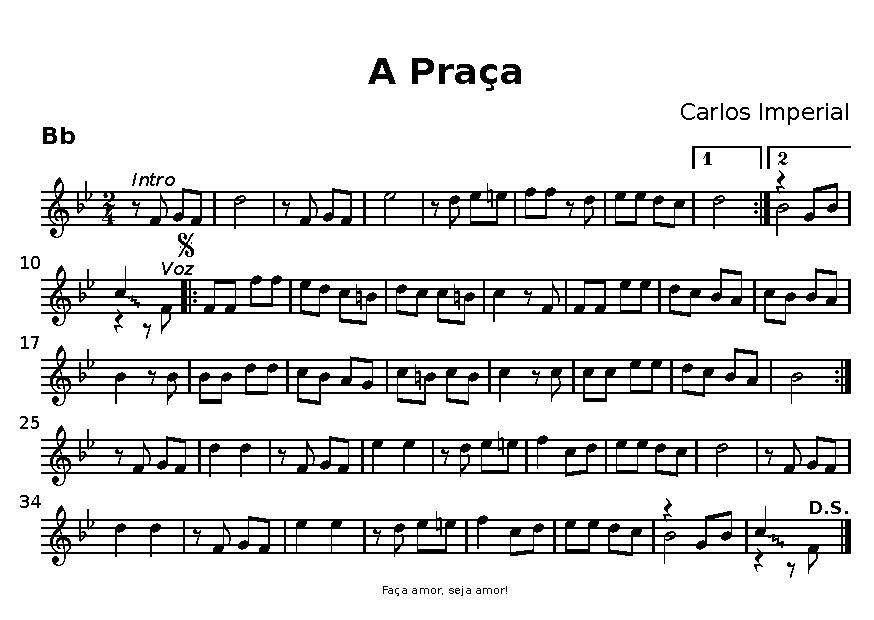
\includepdf{../PDF/aPraca.pdf}

\musica{As Pastorinhas}
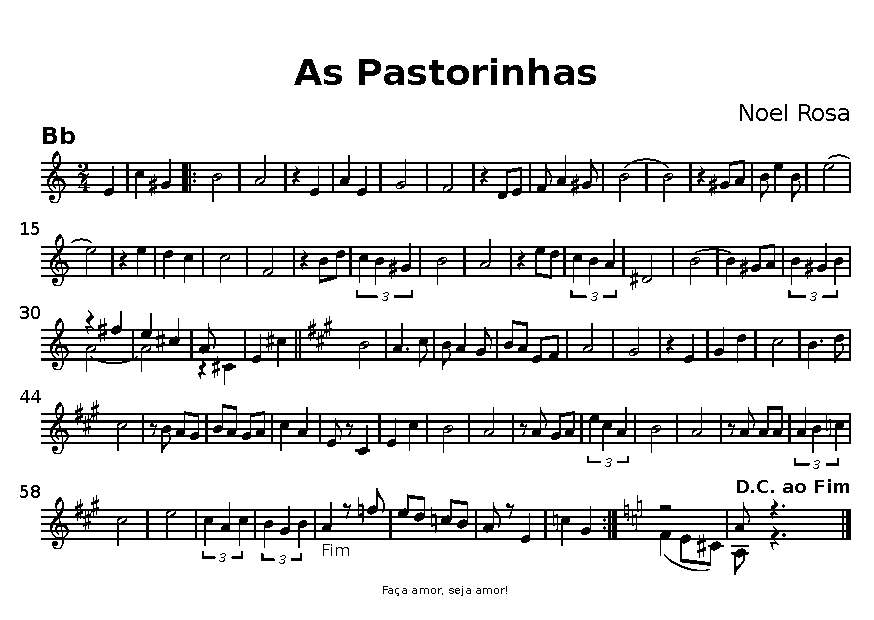
\includepdf{../PDF/pastorinhas.pdf} %Inclui a partitura no songbook
%\musica{Até quarta-feira}
%\musica{Avenida Iluminada}
%\musica{Baile no Municipal}
\musica{Bandeira Branca}
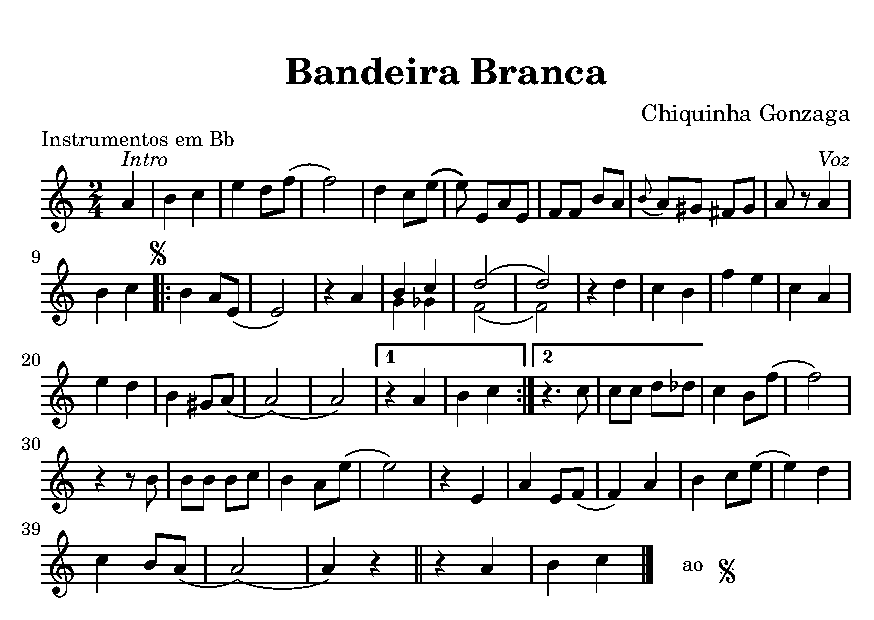
\includepdf{../PDF/bandeiraBranca.pdf}

\musica{Eu quero é botar...}
\includepdf{../PDF/euQueroBotarMeuBloconaRua.pdf}

\musica{Máscara Negra}
\includepdf{../PDF/mascara.pdf}
%\musica{Noite dos mascarados}
\musica{Ô Abre Alas}
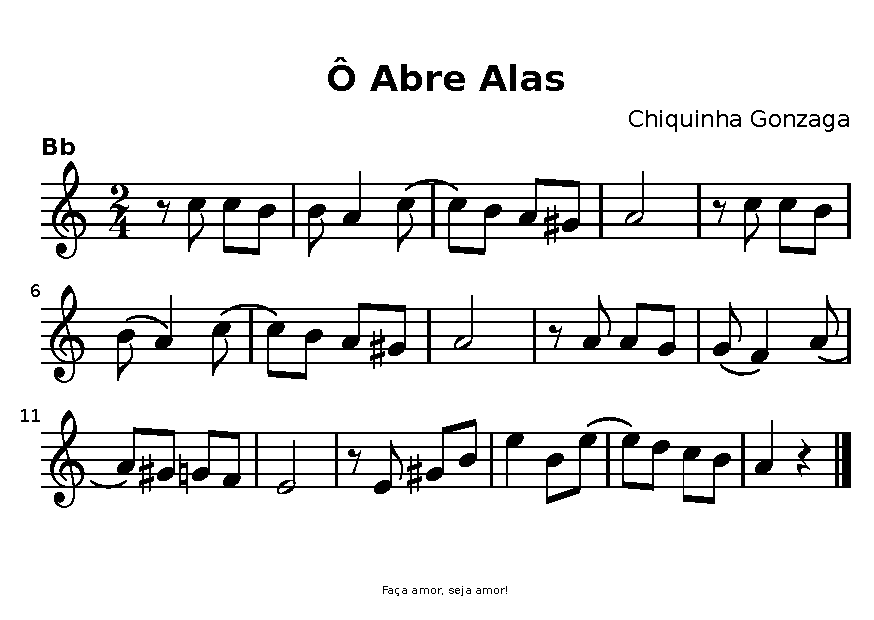
\includepdf{../PDF/abreAlas.pdf}

\musica{Aurora}
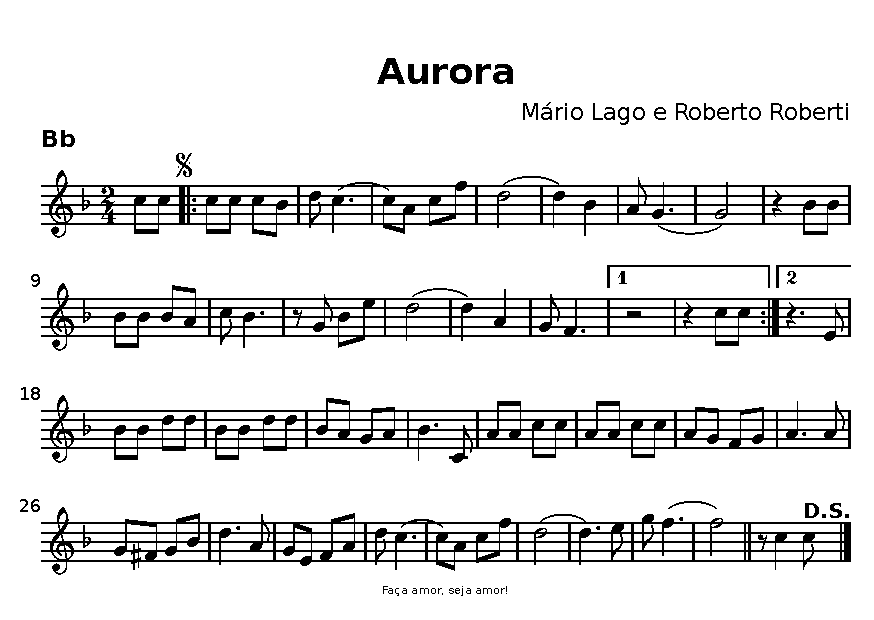
\includepdf{../PDF/aurora.pdf}
% \musica{Balança o saco}
 \musica{Balancê}
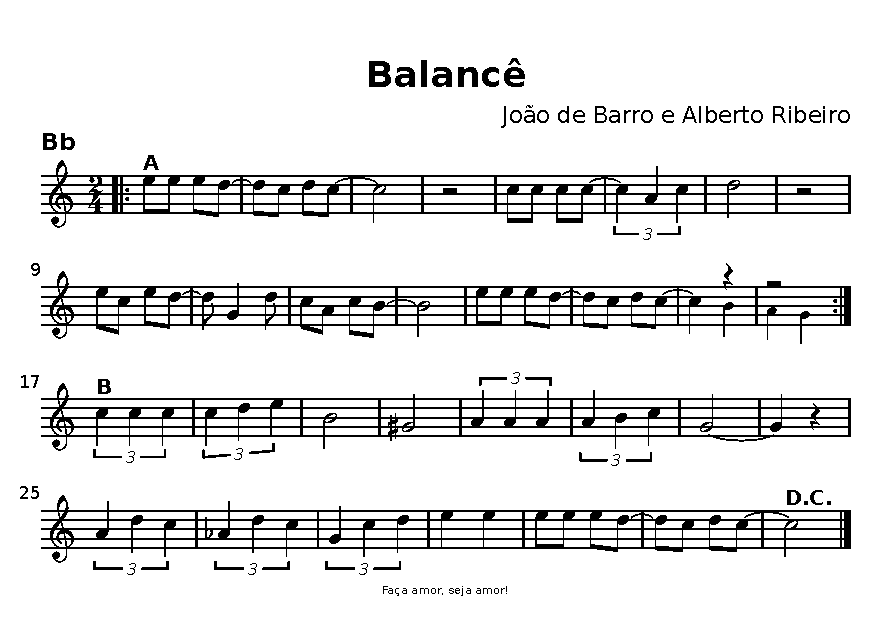
\includepdf{../PDF/balance.pdf}
% \musica{Bota a Camisinha}
\musica{Cabeleira do Zezé}
\includepdf{../PDF/cabeleiraDoZeze.pdf}

\musica{Cachaça}
\includepdf{../PDF/cachaca.pdf}
% \musica{Caiu na rede é peixe}
% \musica{Can Can no Carnaval}

\musica{Coração de Jacaré}
\includepdf{../PDF/coracaoDeJacare.pdf}
% \musica{Daqui não saio}
% \musica{Está chegando a hora}
\musica{Índio quer apito}
\includepdf{../PDF/indio.pdf}

\musica{A Jardineira}
\includepdf{../PDF/jardineira.pdf}

\musica{Mamãe eu Quero}
\includepdf{../PDF/mamaeEuQuero.pdf}

\musica{Marcha da Cueca}
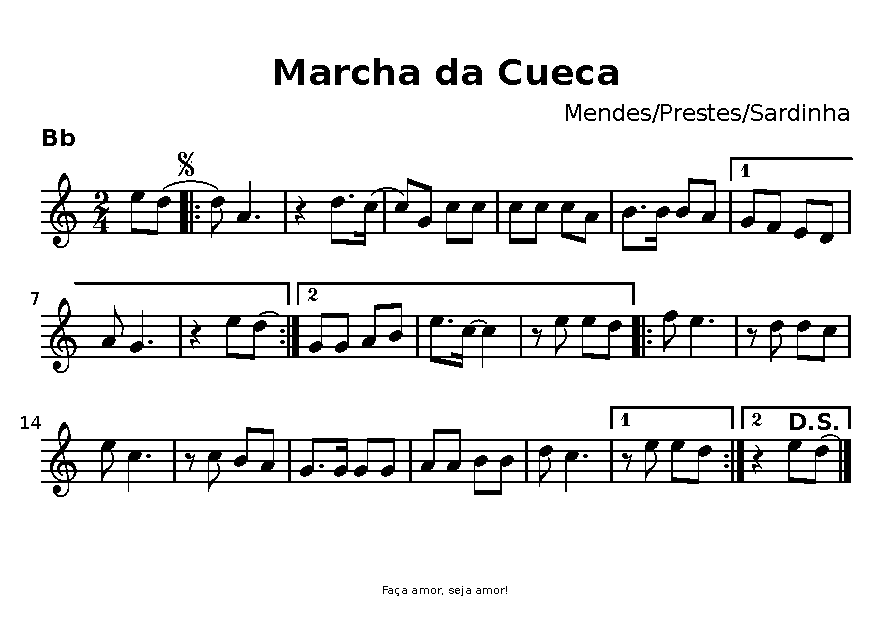
\includepdf{../PDF/marchaDaCueca.pdf}
% \musica{Marcha do Cordão...}

\musica{Marcha do Remador}
\includepdf{../PDF/remador.pdf}

\musica{Maria Sapatão}
\includepdf{../PDF/mariaSapatao.pdf}

\musica{Mulata iê, iê, iê}
\includepdf{../PDF/mulataieieie.pdf}
% \musica{Pegando Fogo}
% \musica{Pescador}

\musica{Saca-Rolha}
\includepdf{../PDF/sacaRolha.pdf}

\musica{Sassaricando}
\includepdf{../PDF/sassaricando.pdf}

\musica{Vai com jeito}
\includepdf{../PDF/vaiComJeito.pdf}

\musica{Marcha da Praia}
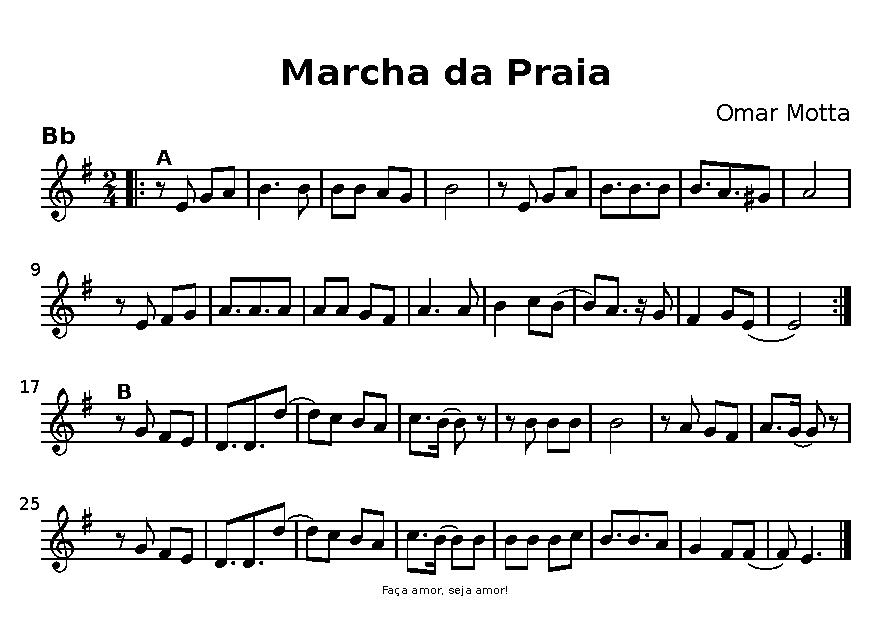
\includepdf{../PDF/praia.pdf} %Inclui a partitura no songbook

\musica{Marcha do Manjericão}
\includepdf{../PDF/manjericao.pdf}


%\musica{Água Mineral}
%\musica{Alô Paixão}
%\musica{Baianidade Nagô}
%\musica{Beija-Flor}
%\musica{Beleza Rara}
%\musica{Berimbau Metalizado}
%\musica{Boquinha da garrafa}
%\musica{Céu da boca}
%\musica{Cordeiro de Nanã}
%\musica{De Ladinho}
%\musica{Eu também quero beijar}
%\musica{Libera Geral}
%\musica{Me abraça, me beija}
%\musica{Mila}
%\musica{Nossa gente (Avisa lá)}
%\musica{O canto da cidade}
%\musica{Prefixo do Verão}
\musica{Requebra}
\includepdf{../PDF/requebra.pdf}
%\musica{Requebra }
%\musica{Sexy Iemanjá}

\musica{Anunciação}
\includepdf{../PDF/anunciacao.pdf}
%\musica{La belle du jour}
%\musica{Girassol}
%\musica{Morena Tropicana}
%\musica{Acorda Maria Bonita}
\musica{Qui Nem Jiló}
\includepdf{../PDF/quiNemJilo.pdf}
%\musica{Fui Fiel}
%\musica{Porque Homem não chora}

%\musica{Lindo Lago do Amor}
%\musica{Atras do trio elétrico}
%\musica{Banho de cheiro}
%\musica{Bloco do Prazer}
%\musica{Não existe pecado ao...}
%\m
\musica{Cilada}
\includepdf{../PDF/cilada.pdf}
%\musica{Ê baiana}
%\musica{Kid Cavaquinho}
%\musica{Recordar é viver}
%\musica{Trem das Onze}
%\musica{Tristeza}

%\musica{Morto muito louco}
%\musica{Rap da Felicidade}
%\musica{Rap das Armas}
%\musica{Show das poderosas}


%\musica{Acenda o farol}
%\musica{Azul da cor do mar}
%\musica{Batata frita}
%\musica{Bom senso}
%\musica{Canário do Reino}
%\musica{Chove Chuva}
%\musica{Contato com o Mundo\\Flores Belas}
%\musica{Cristina}
%\musica{Ela partiu}
%\musica{Fio Maravilha}
%\musica{Gostava tanto de você}
%\musica{Guiné Bissau...}
%\musica{Imunização Racional...}
%\musica{Ive Brussel}
%\musica{Márcio Leonardo e Telmo}
%\musica{Menina mulher}
%\musica{Meus Filhos\\Que beleza}
%\musica{Não quero dinheiro}

%\musica{Primavera}
%\musica{Quem cochicha...}
%\musica{Sossego}
%\musica{Taj Mahal}
%\musica{Terapêutica do grito}
%\musica{Umbabarauma}

\musica{Superfantástico}
\includepdf{../PDF/superfantastico.pdf}
%\musica{Uma brasileira}
%\musica{Aflorou}

\end{document}
